\chapter{La Historia Clinica}

\section{El Problema}

Actualmente las Historias clinicas de cada paciente se almacenan en documentos
impresos semi formateados (Como se puede Observar en las Figuras 3.1 y 3.2)
y rellenados manualmente por el personal de la
institucion, lo cual genera varios problemas tanto de almacenamiento ya que cuanto
mas crece el numero de pacientes se necesita ampliar el espacio fisico requerido
para almacenar su imformacion mediantes ficheros, El acceso a la informacion
y la busqueda de los antecedentes de un paciente suele ser demaciada lenta
por el volumen de ficheros que la persona debe revisar para localizar el
archivo requerido. 

\begin{figure}[h]
    \centering
    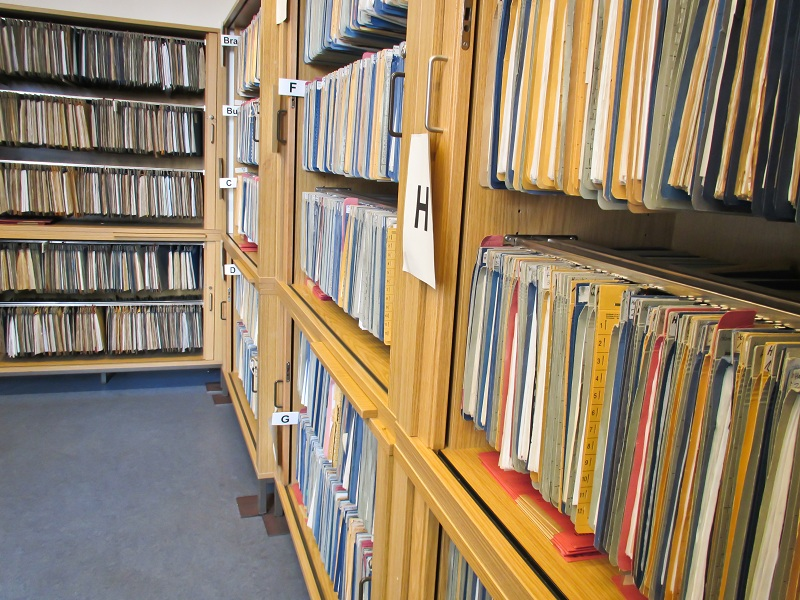
\includegraphics[scale=1.5]{resourse/folders-archivos.jpg}
    \caption{Almacenamiento Fisico de Archivos}
    \label{fig:05}
\end{figure}  


\begin{figure}[H]
    \centering
    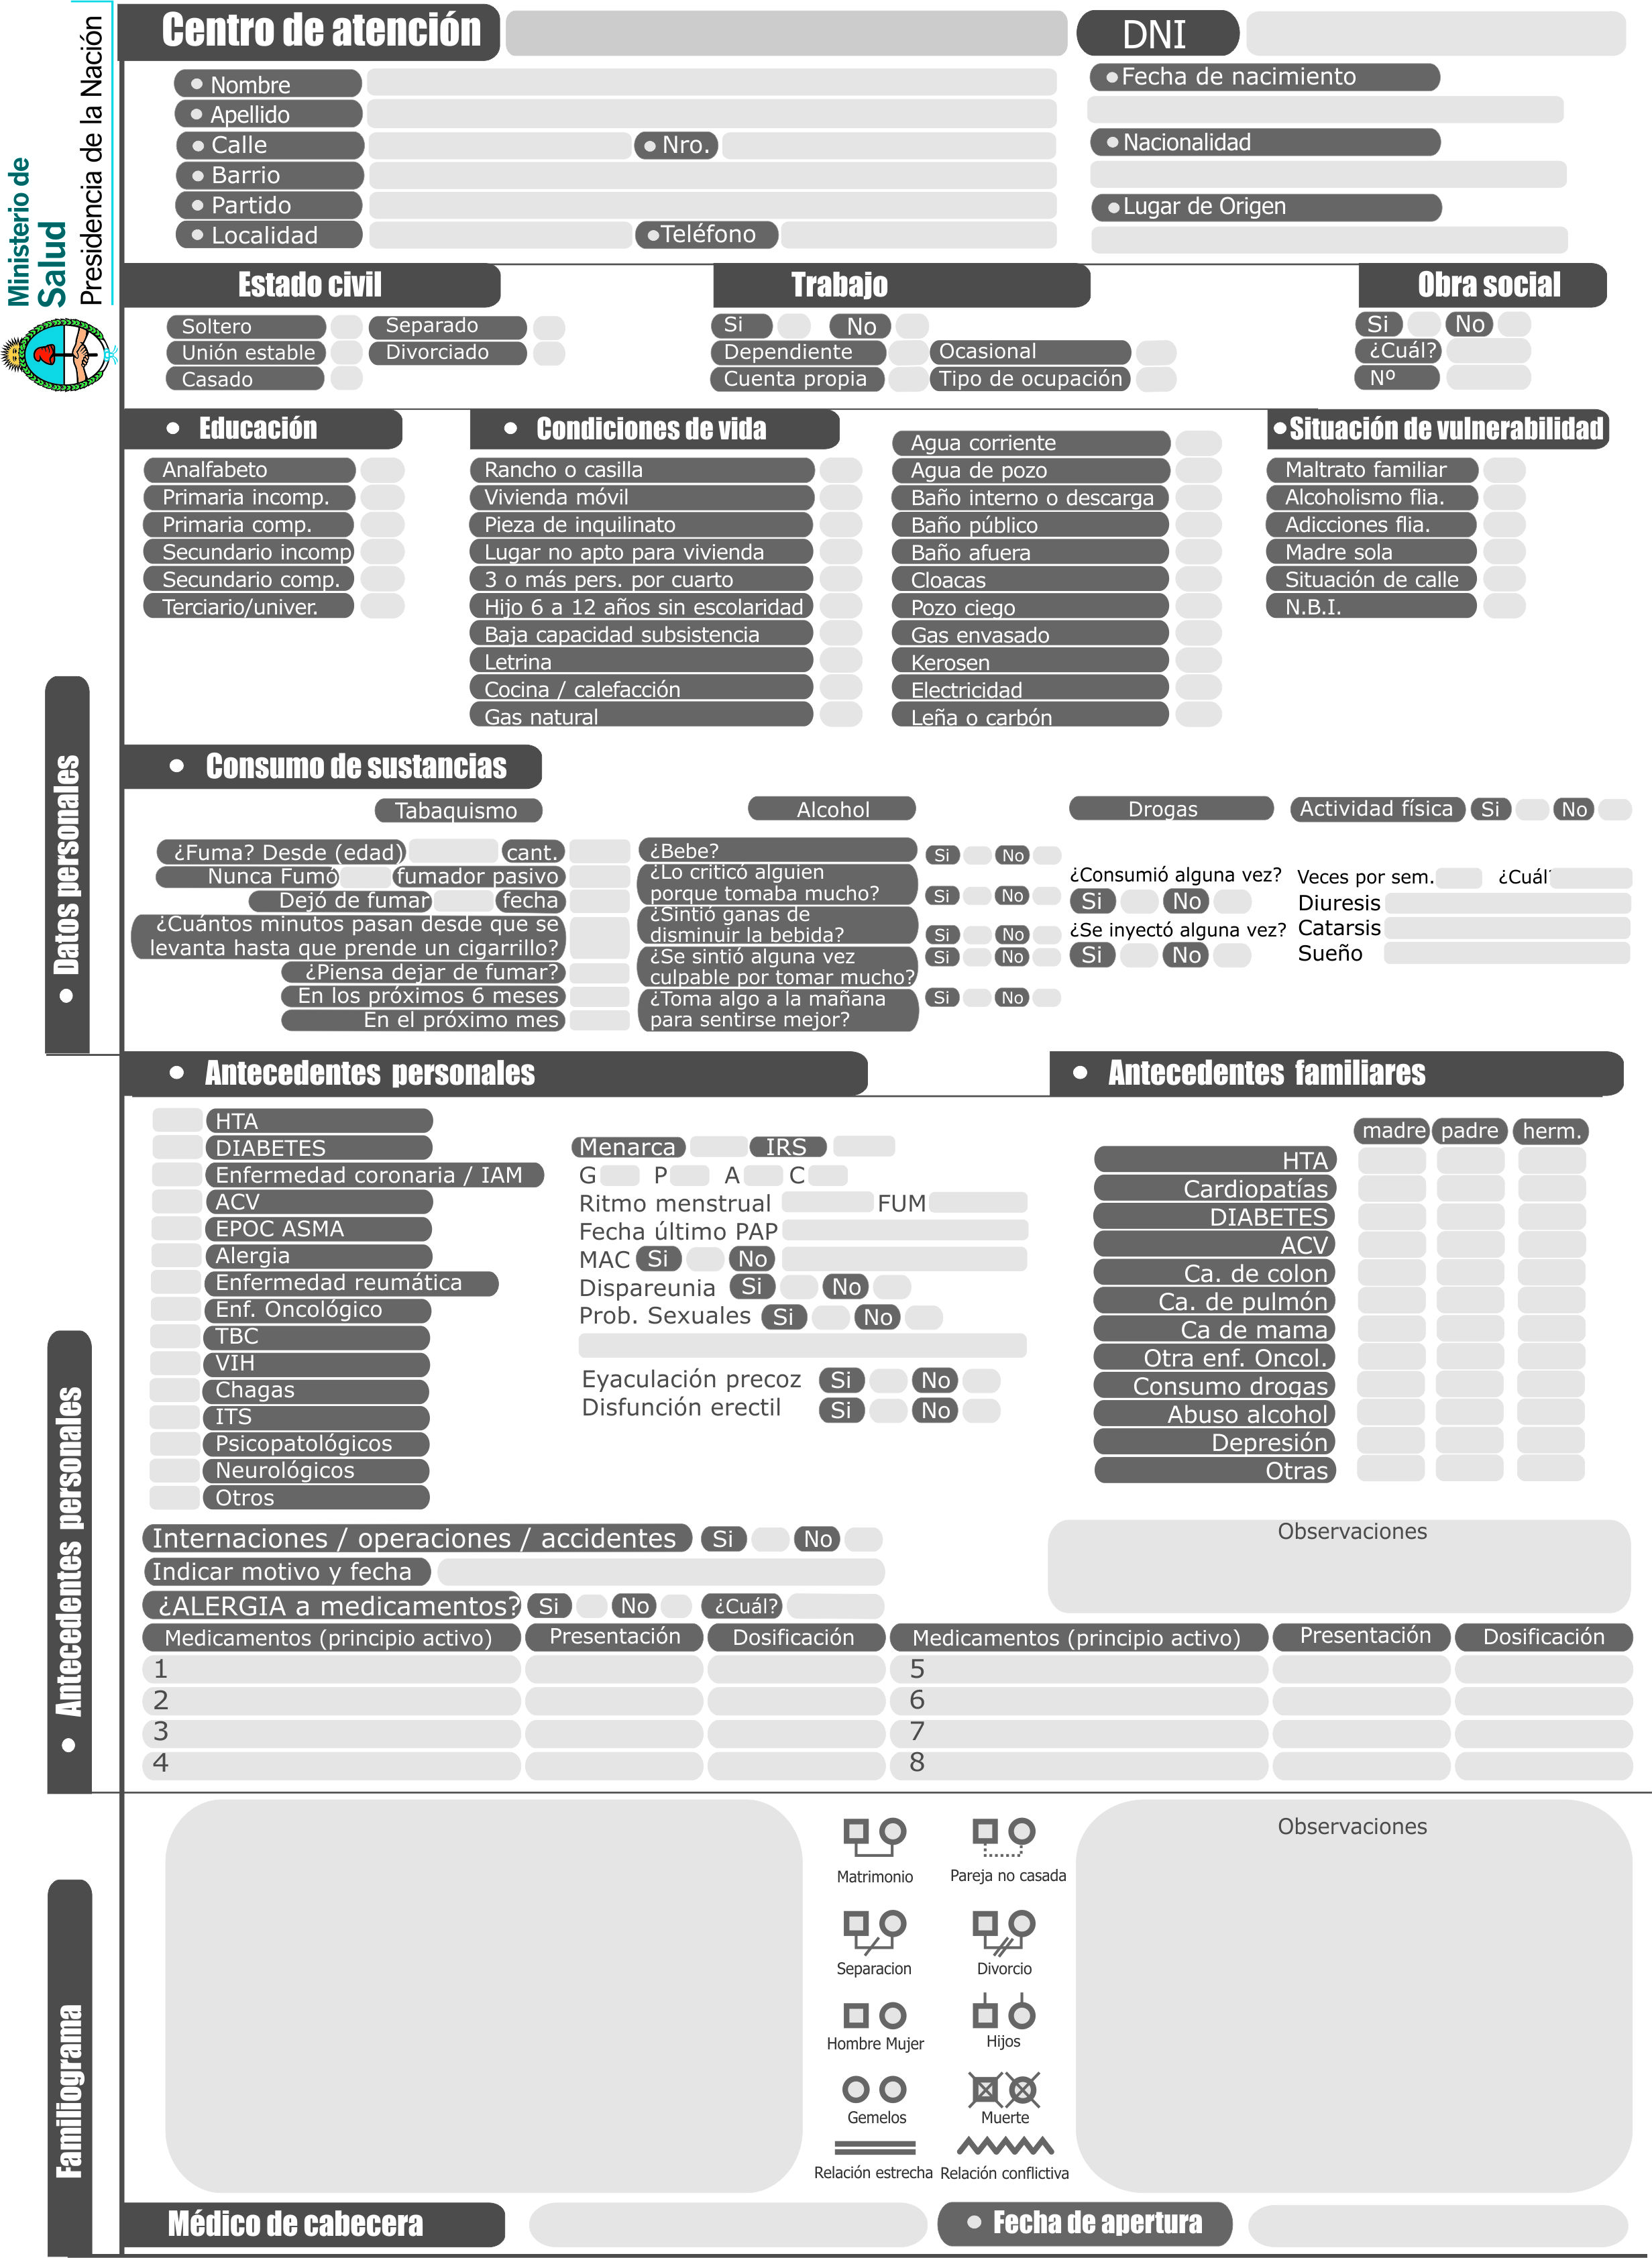
\includegraphics[scale=0.7]{resourse/historia-clinica-f.jpg}
    \caption{Modelo Historia Clinica Ministerio de Salud de La Nacion Pag 1}
    \label{fig:06}
\end{figure}  

\begin{figure}[H]
    \centering
    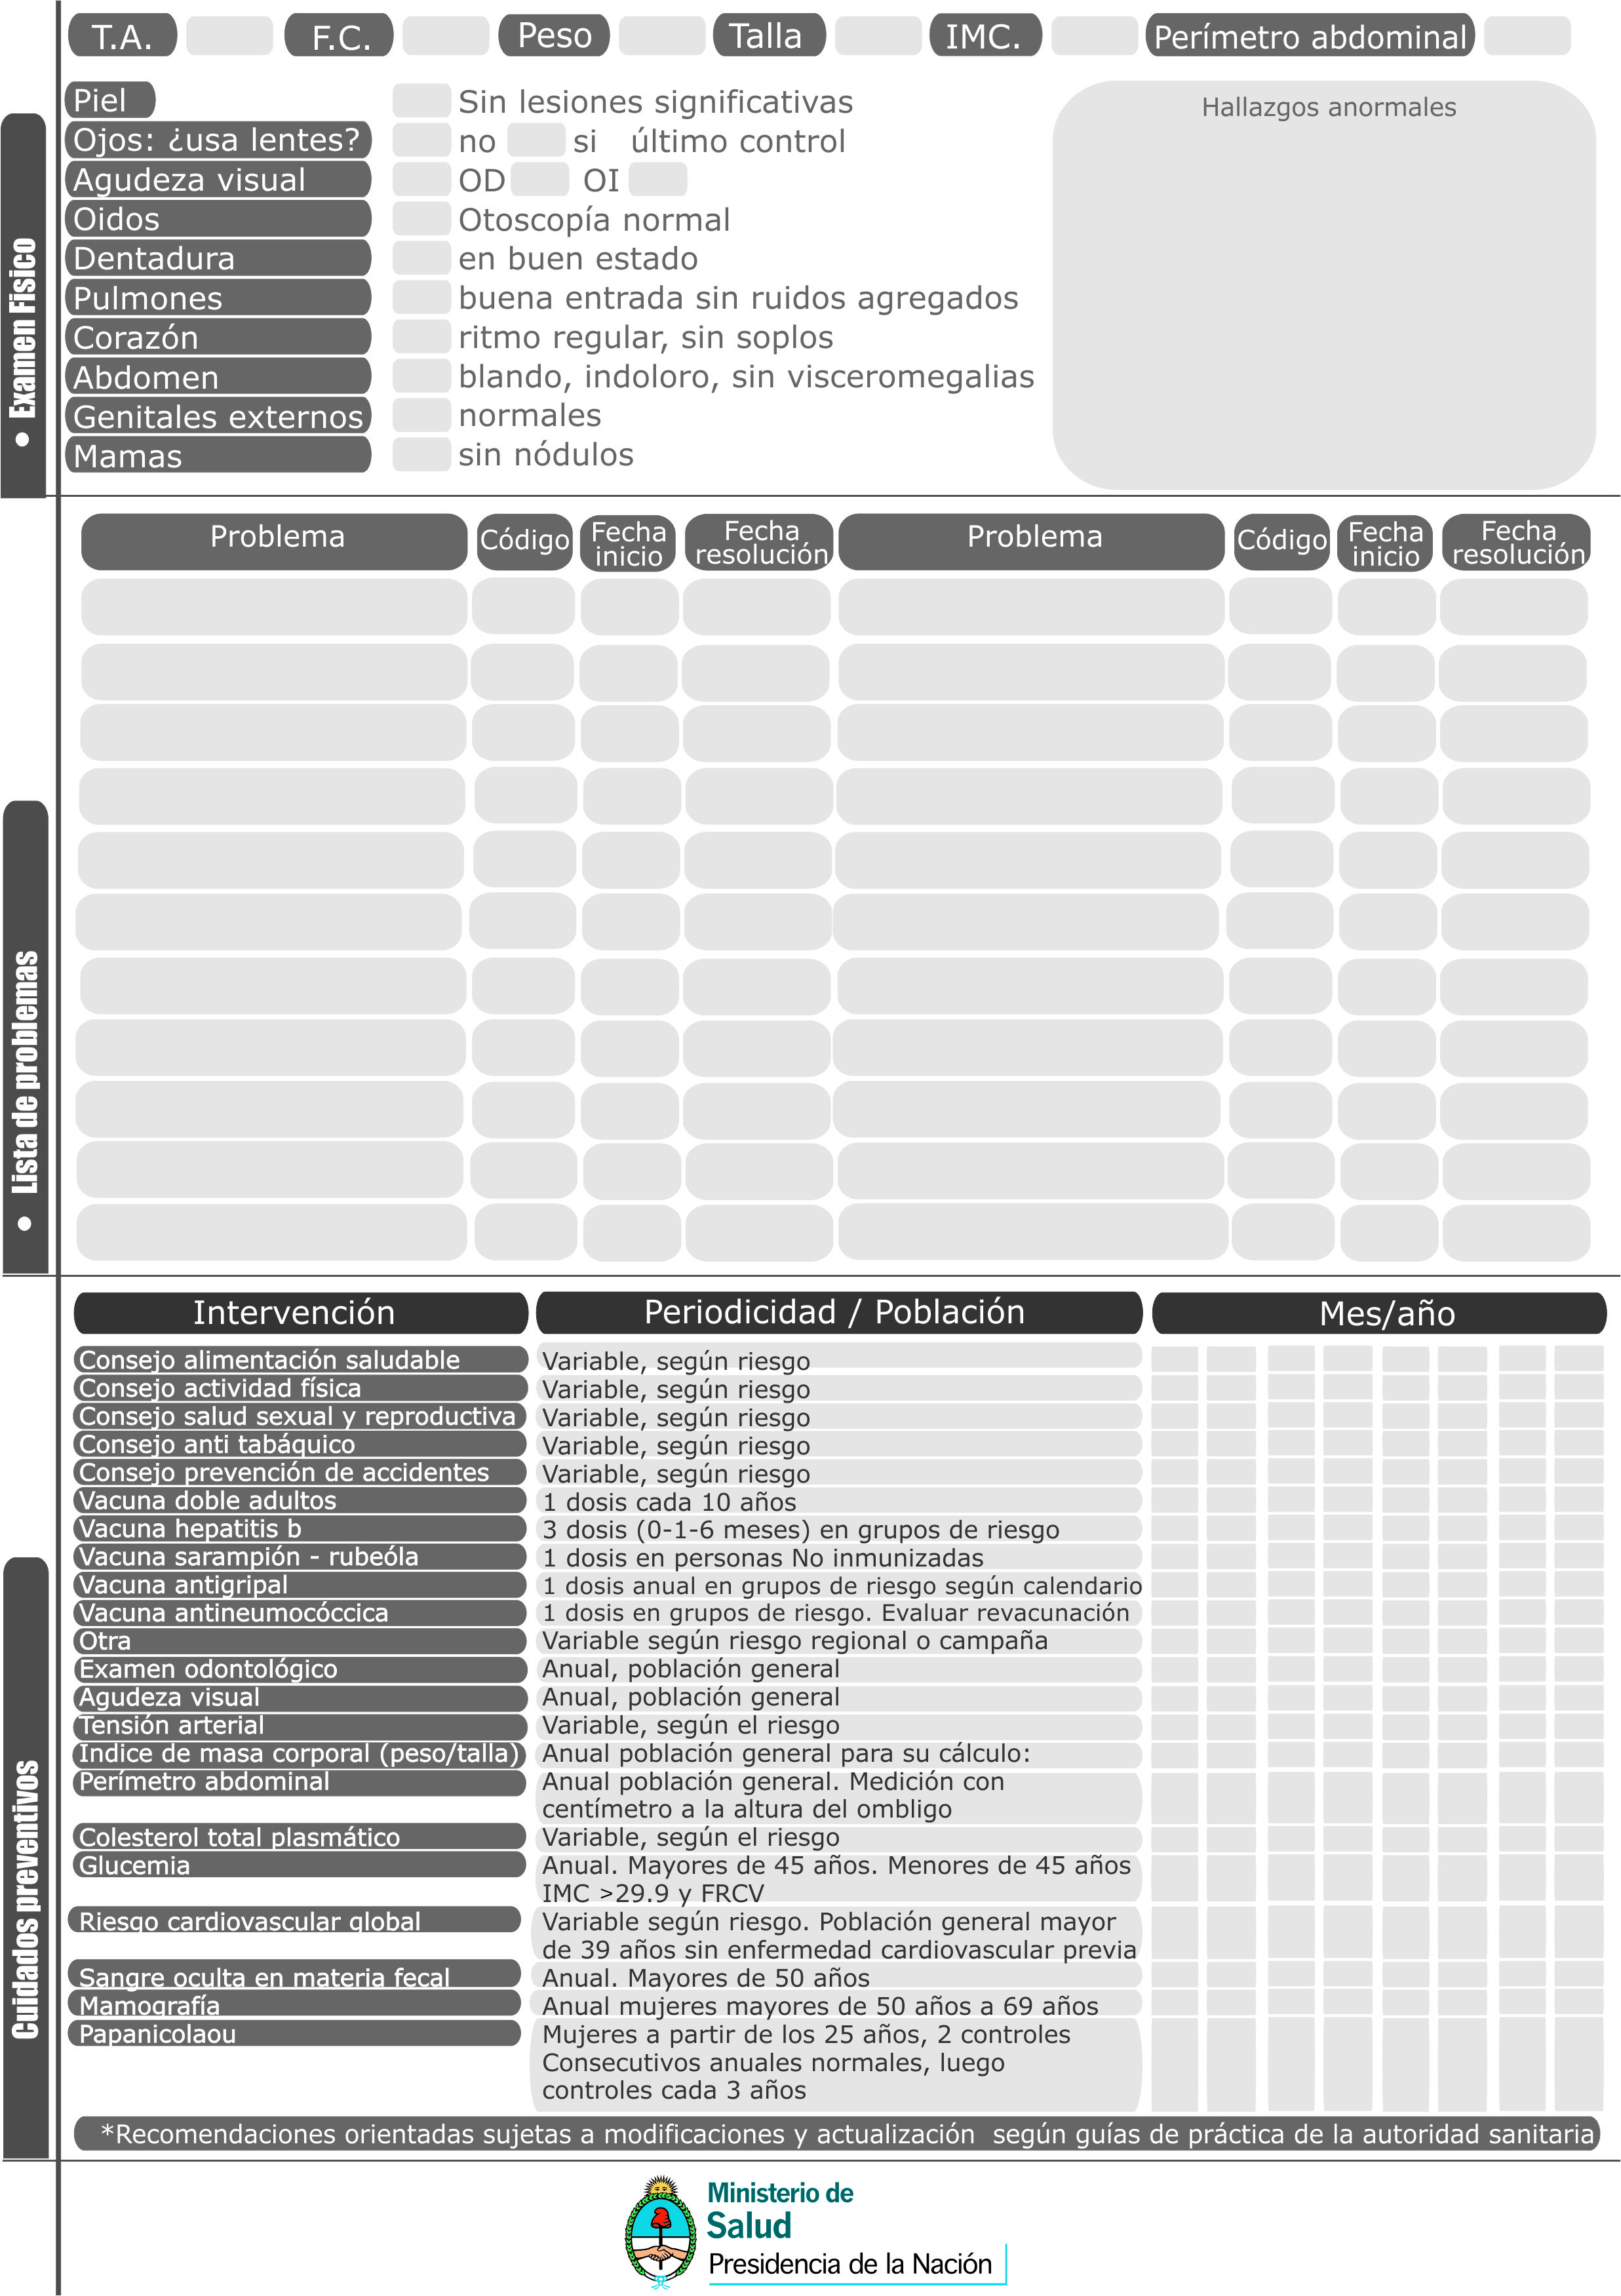
\includegraphics[scale=0.7]{resourse/historia-clinica-d.jpg}
    \caption{Modelo Historia Clinica Ministerio de Salud de La Nacion Pag 2}
    \label{fig:07}
\end{figure}  




\section{La Solucion}

Por ello este era un ecenario perfecto donde Es Necesario informatizar el
Actual Sistema, lo cual solucionaria los 2 principales problemas del mismo
que son el Excesivo espacio de almacenamiento y el lento trabajo de busqueda
ademas de:

\begin{itemize}
    \item Reducir costos de Personal Administrativo, ya que las busquedas y registro las hara el Sistema.
    \item Brindar la informacion de manera rapida en situaciones criticas que requieren un rapido accionar por parte del
    Medico.
    \item Disponibilidad En todo momento y cualquier lugar para consulta por parte de los Medicos ya que solo requerira
        disponer de un usuario y un ordenador con coneccion a Internet para poder consultar.
\end{itemize}

\begin{figure}[H]
    \centering
    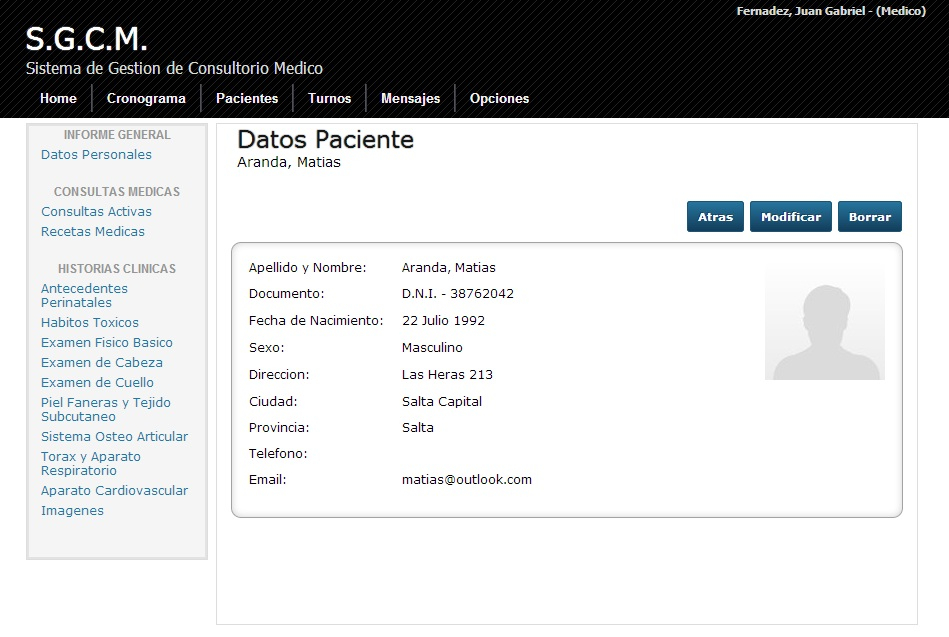
\includegraphics[scale=0.7]{resourse/sist-hist-clin.jpg}
    \caption{Pantalla Presentacion Historia Clinica}
    \label{fig:08}
\end{figure}  

\footnote{Nota: Los datos de pacientes que se muestran son a modo Ejemplo no pertenecen a personas reales}
